\begin{frame}{Agenda}
	In this presentation
	\begin{enumerate}
		\item Introduction \& motivation
		\item Overview of contributions
		\item Specifics of contribution 1
		\item Specifics of contribution 2
		\item Conclusion \& discussion
	\end{enumerate}
\end{frame}

\begin{frame}{Introduction}
	\begin{columns}
		\column{0.25\textwidth}

		
\includegraphics[width=0.95\textwidth]{../delft-style/title/logos/nedtrain}

		\bigskip

		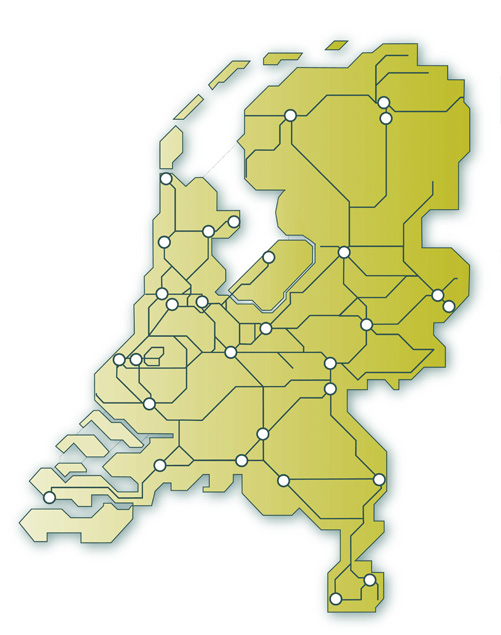
\includegraphics[width=0.95\textwidth]{spoornet-kaart}

		\column{0.75\textwidth}

		Scheduling of operations, or tasks, or activities, under uncertainty

		\medskip

		Inspired by a real-world problem as experienced by NedTrain
		\begin{itemize}
			\item That part of NS that handles fleet-maintenance 
			\item Maintenance workshops distributed over the Netherlands
		\end{itemize}
	\end{columns}
\end{frame}

\begin{frame}{Introduction - in the workshop}
	The weekly scheduling process
	\begin{itemize}
		\item Thousands of maintenance tasks over several trains
		\item Resources: people, equipment, platforms, etc.
		\item Train delivery deadlines
	\end{itemize}

	\bigskip

	Human resources organized into autonomous teams 
	\begin{itemize}
		\item Members of a team can communicate freely
		\item Cross-team communication is an issue
	\end{itemize}
\end{frame}

\begin{frame}{Scheduling complications}
	Uncertainty complicates scheduling
	\begin{itemize}
		\item Conditional repair tasks
		\item Uncertain task durations: \\
			$\rightarrow$ how much time to allocate? $\rightarrow$ when to start?
	\end{itemize}

	\medskip

	\begin{center}
		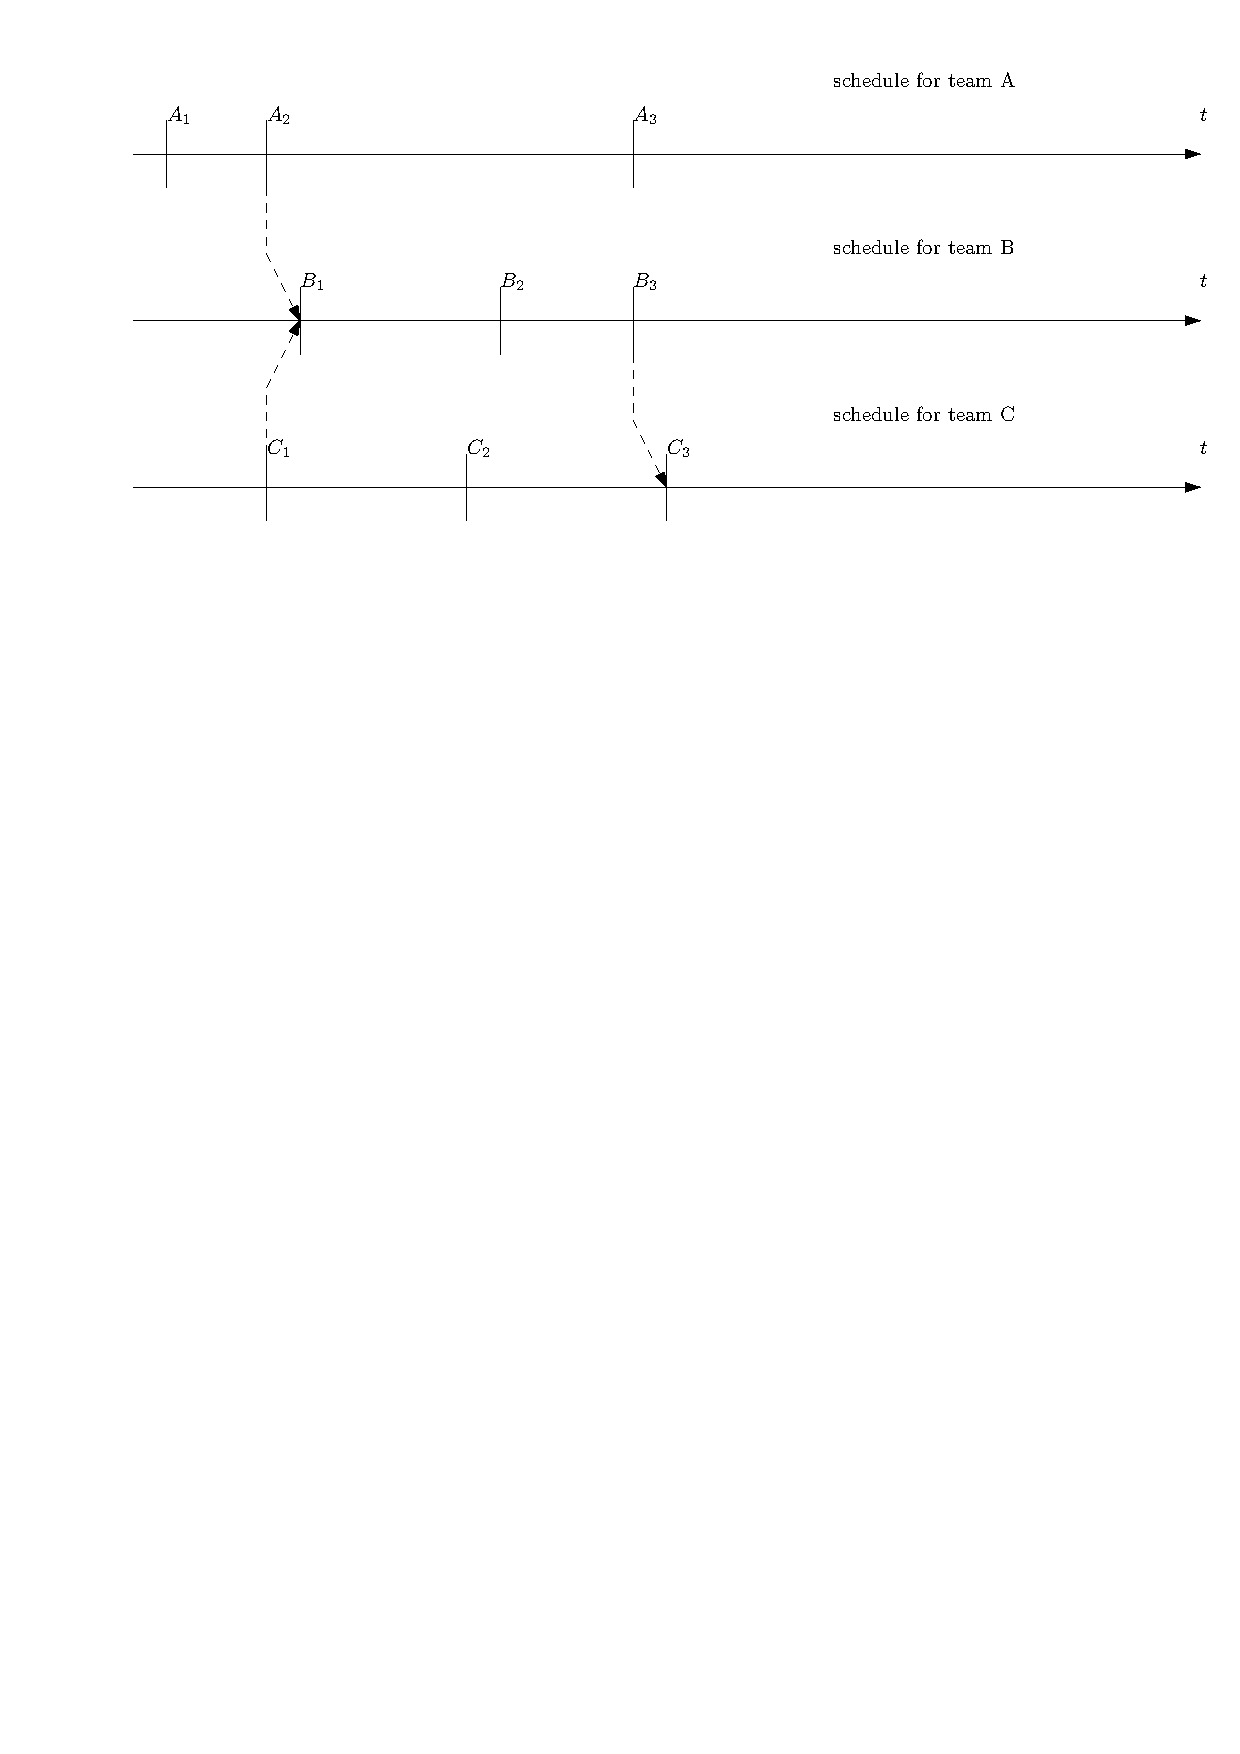
\includegraphics[width=0.8\textwidth]{team-schedules}
	\end{center}

	\medskip

	\only<2>{\st{Schedule by hand and keep adapting accordingly}}
\end{frame}

\begin{frame}{Our contributions}
	\st{Schedule by hand and keep adapting accordingly}
	\begin{itemize}
		\item People hate to be directed by a schedule that changes repeatedly 
		\item Deadlines are compromised
	\end{itemize}

	\bigskip

	We contribute two scheduling techniques:
	offer management two alternatives for dealing with the aforementioned scheduling challenges
	\begin{enumerate}
		\item Let people reschedule themselves at will \\
			\ldots ~ but ensure no conflicts in autonomous decisions

		\item Do create a schedule that directs people \\
			\ldots ~ but ensure it remains unchanged during execution
	\end{enumerate}
\end{frame}

\begin{frame}{Approach 1}
	%instead of a regular schedule we assign each ask with a window in time 
	%such an assignment of time-windows to tasks, we call a flexible schedule and it facilitates a temporal decoupling
	Create a ``flexible'' or ``interval'' schedule, instead of a regular schedule
	\begin{itemize}
		\item assigns a time-window to each task
		\item facilitates a ``temporal decoupling''
	\end{itemize}

	\pause
	\medskip

	Teams can freely choose within the provided time-windows 
	\begin{itemize}
		\item no need to account for choices of other teams
		\item scheduling constraints always satisfied
	\end{itemize}
	
	%teams can freely choose within the provided time-windows without having to worry about the choices of other teams
	%we ensure scheduling constraints will be satisfied so long as tasks are executed within their appointed time-windows

	\medskip

	Objective: maximize the amount of ``flexibility'' offered (i.e. width of those time-windows)
\end{frame}

\begin{frame}{Approach 1 -- example}
	Objective: maximize the amount of ``flexibility'' offered (i.e. width of those time-windows)

	\bigskip
	\begin{center}
		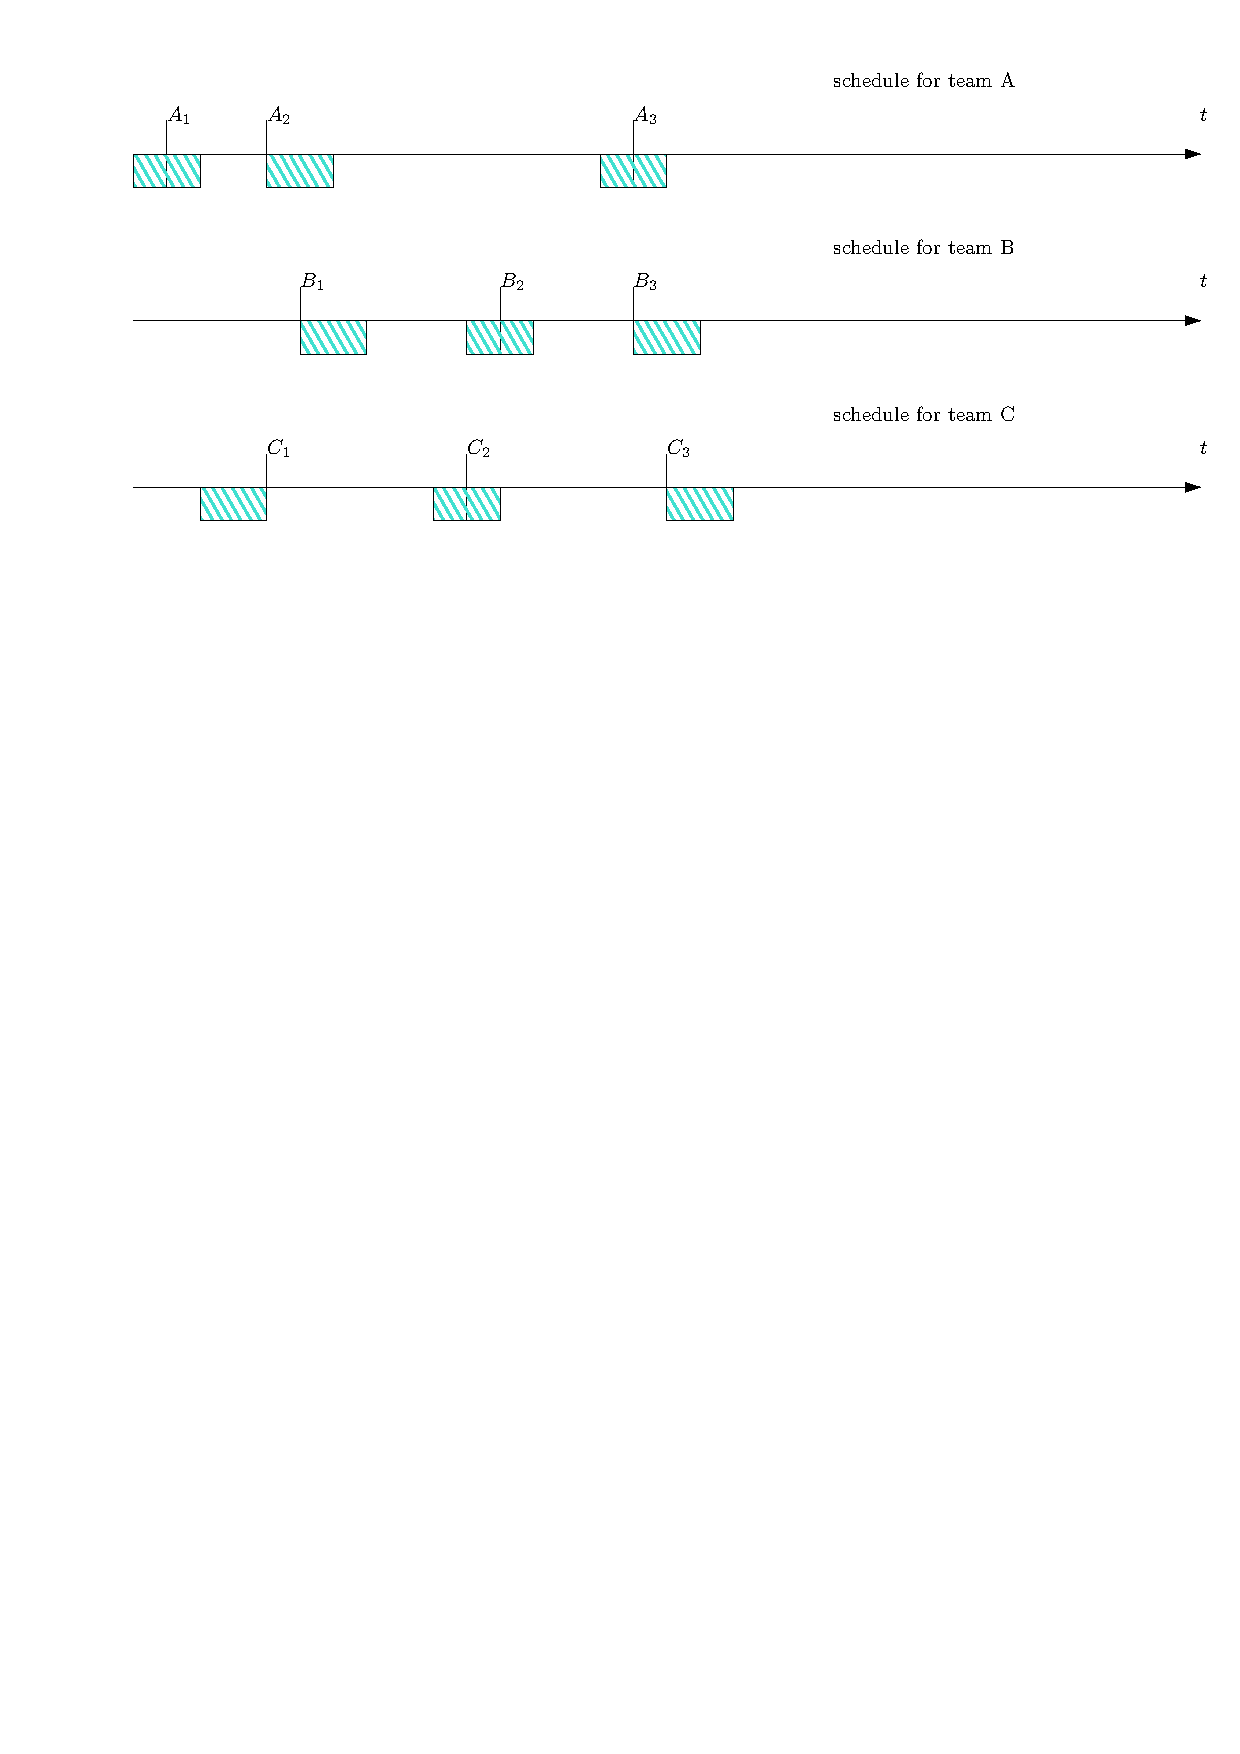
\includegraphics[width=0.9\textwidth]{team-schedules2}
	\end{center}
\end{frame}

\begin{frame}{Approach 2}
	%disadvantage of the first approach is that we don't make use of an interesting fact:
	%tasks appear periodically; each type of task appears repeatedly through different maintenance weeks and different trains
	First approach does not make use of the following:
	\begin{itemize}
		\item Variety of maintenance tasks is limited
		\item We have a ``sample'' of task durations
	\end{itemize}

	\medskip

	Durations are uncertain but not completely unpredictable!

	\pause

	Example
	\bigskip
	\begin{center}
		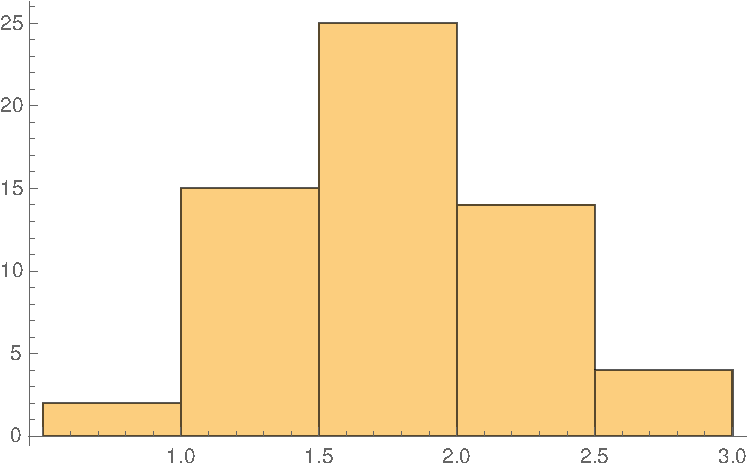
\includegraphics[width=0.6\textwidth]{histo}
	\end{center}
\end{frame}


\begin{frame}{Approach 2}
	Main idea:\\
	Use data from past sessions to model task durations as random variables with a distribution

	\medskip

	%based on this stochastic modelling uncertainty in the workshop
	%generate a schedule, this time a regular schedule, that is stable and robust 
	Create a (regular) schedule that is ``stable'' and ``robust'' \\
	\ldots for this \emph{particular} model of uncertainty
	\begin{itemize}
		\item stable: it won't change much
		\item robust: trains will most likely be delivered on time
	\end{itemize}

	\medskip
	Leverage precise knowledge of uncertainty to allocate ``slack''
\end{frame}

\begin{frame}{Approach 2 -- example}
	Leverage precise knowledge of uncertainty to allocate ``slack''

	\bigskip

	\begin{center}
		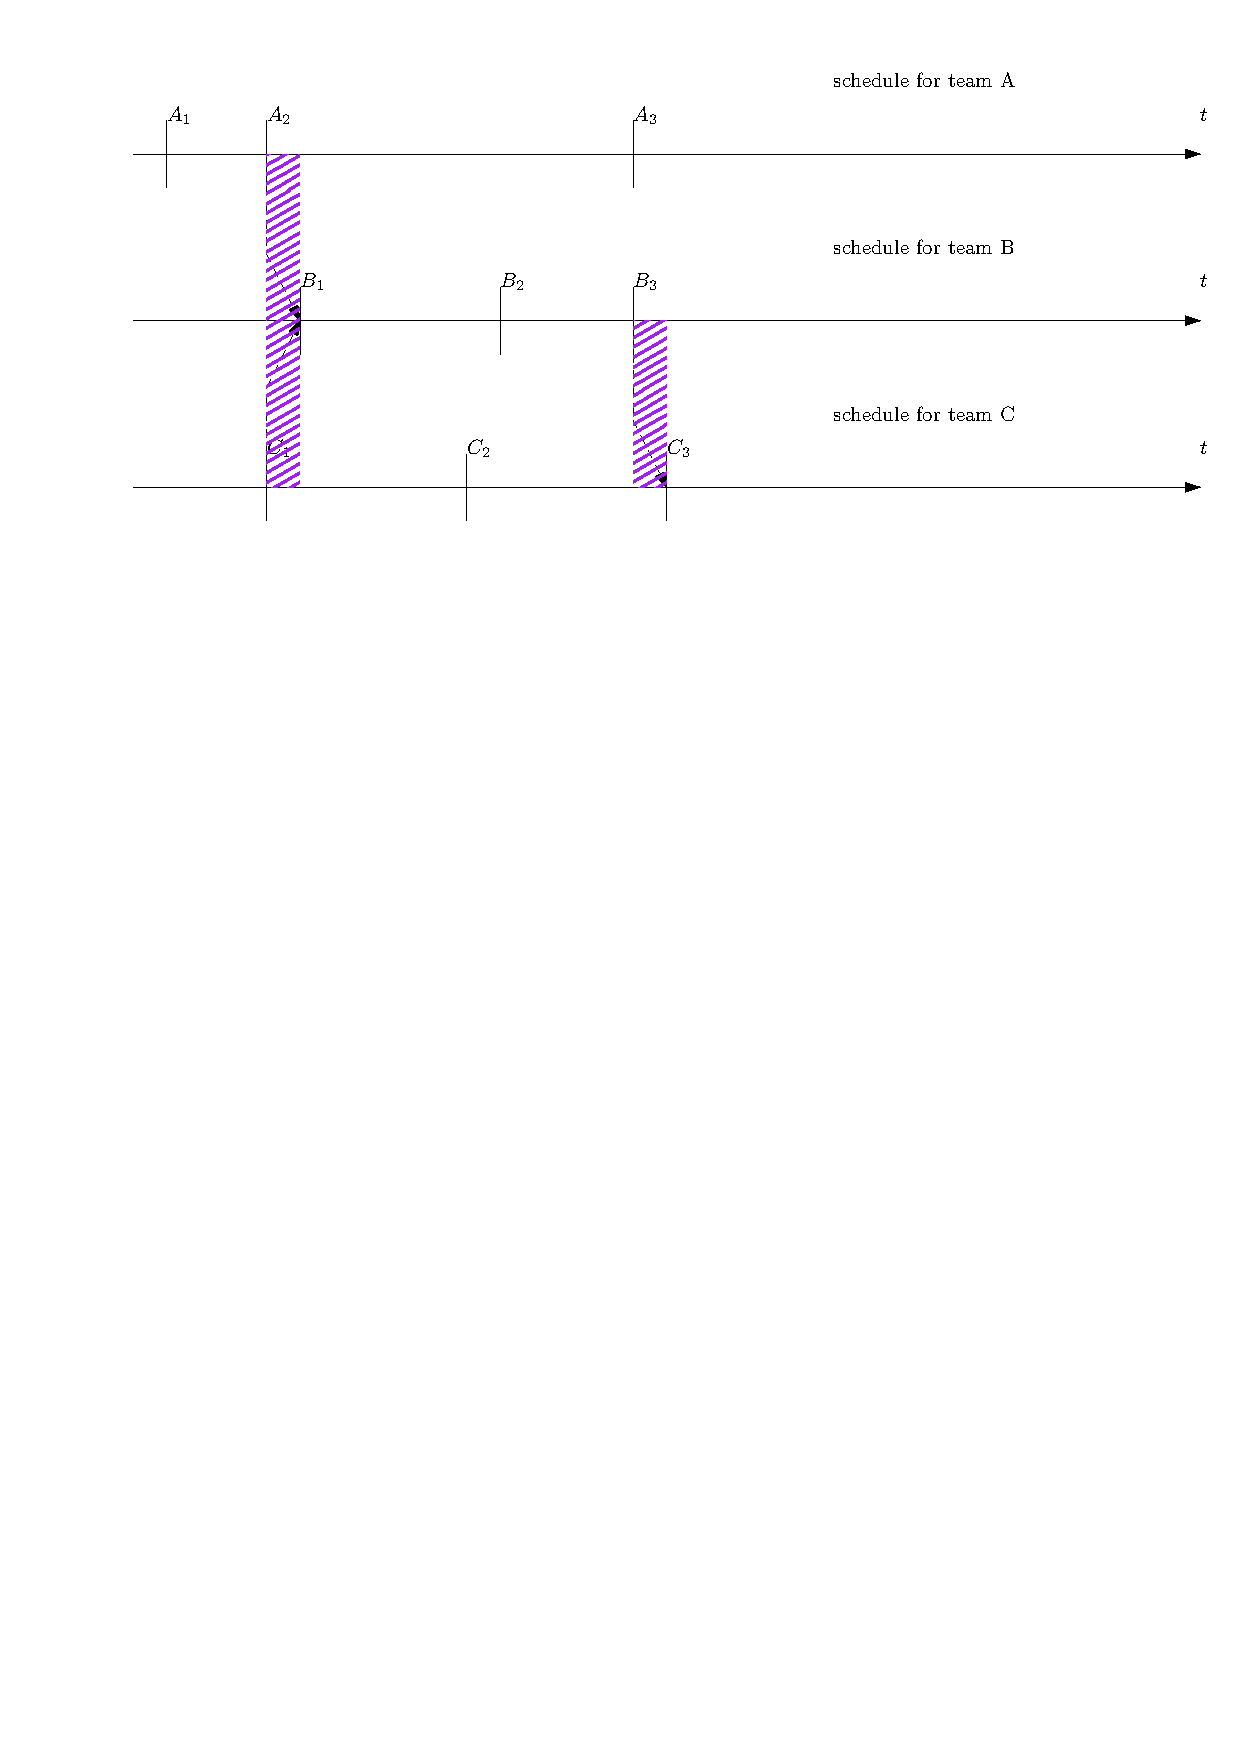
\includegraphics[width=0.9\textwidth]{team-schedules3}
	\end{center}
\end{frame}


\begin{frame}{Conclusion \& Discussion}
	Flexible schedules vss. Robust/stable schedules?
	\begin{itemize}
		\item Needs further discussion
		\item Finding the answer might be a project in itself
	\end{itemize}

	\medskip

	Our work is not necessarily NedTrain-specific

	\pause
	\medskip

	Future work
	\begin{itemize}
		\item Try to combine the two approaches
		\item Experiment with NedTrain data
		\item Other
		\begin{itemize}
			\item Variations of flexible schedules (``provisional'' schedules)
			\item How to ``help'' flexibility by careful allocation of resources to tasks
			\item Team-level, instead of task-level, temporal decoupling
		\end{itemize}
	\end{itemize}
\end{frame}
	
